% Chapter Template

\chapter{MCC and SARSA plots side by side with the same card coding} % Main chapter title

\label{MCC and SARSA plots side by side with the same card coding} % Change X to a consecutive number; for referencing this chapter elsewhere, use \cref{ChapterX}

\begin{itemize}
    \item MCC with 10'\,000'\,000 episodes
    \item SARSA with 1'\,000'\,000 episodes
\end{itemize}

\vspace{2cm}

\begin{figure}[ht!]
    \begin{subfigure}{0.5\textwidth}
        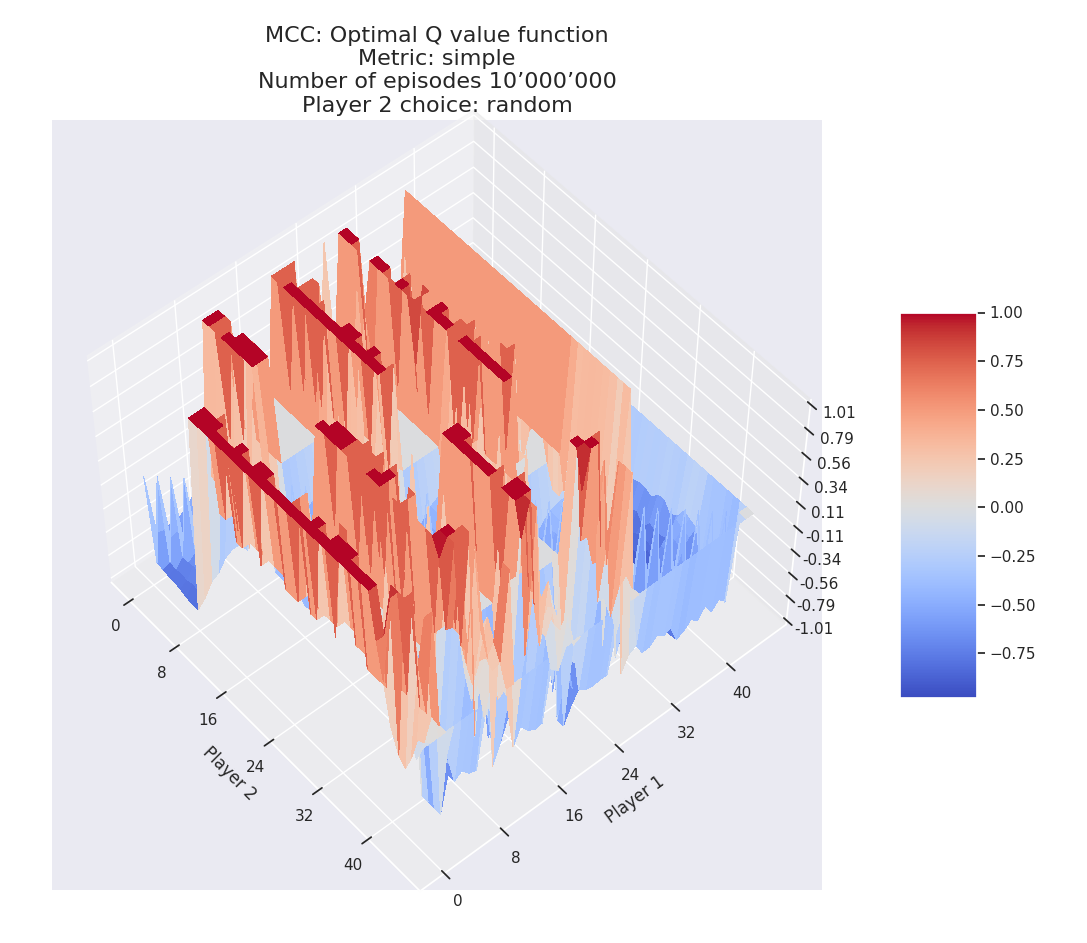
\includegraphics[width=1\linewidth]{Figures/mcc_simple_10000000_random} 
        \caption[MCC simple]{MCC simple}
        \label{fig:mcc simple}
    \end{subfigure}
    \begin{subfigure}{0.5\textwidth}
        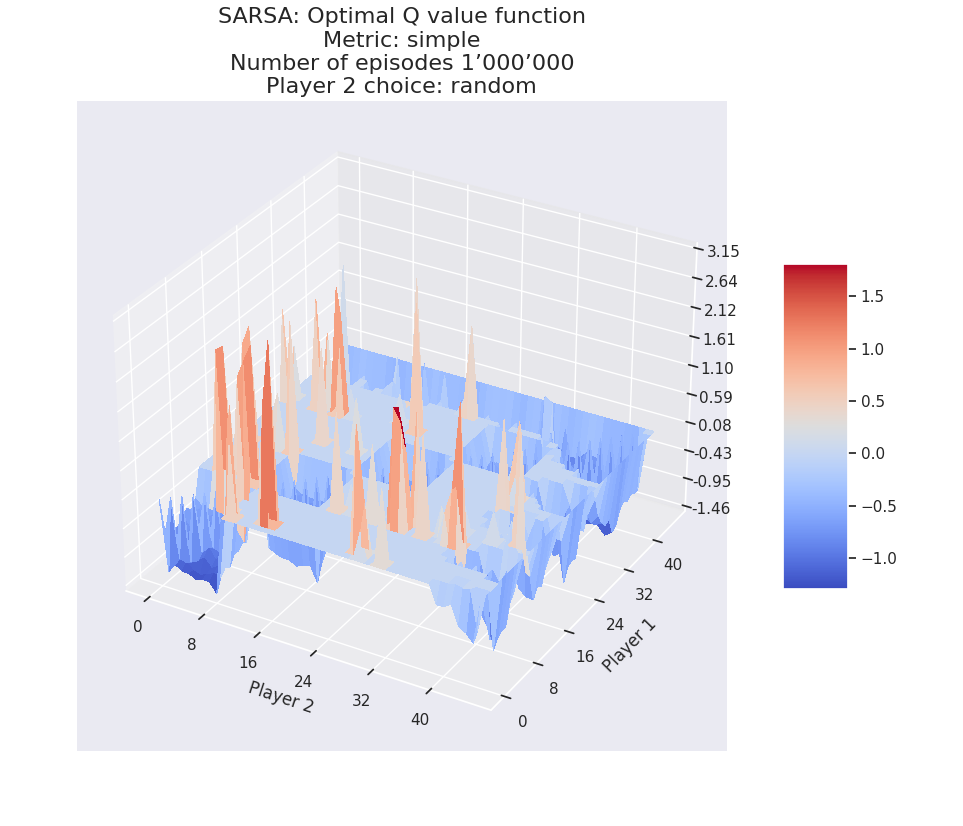
\includegraphics[width=1\linewidth]{Figures/SARSA_simple_1000000_random}
        \caption[SARSA simple]{SARSA simple}
        \label{fig:sarsa simple}
    \end{subfigure} \\
    \caption{MCC and SARSA card encoding: simple}
\label{fig:MCC and SARSA card encoding: simple}
\end{figure}

\begin{figure}[ht!]
    \begin{subfigure}{0.5\textwidth}
        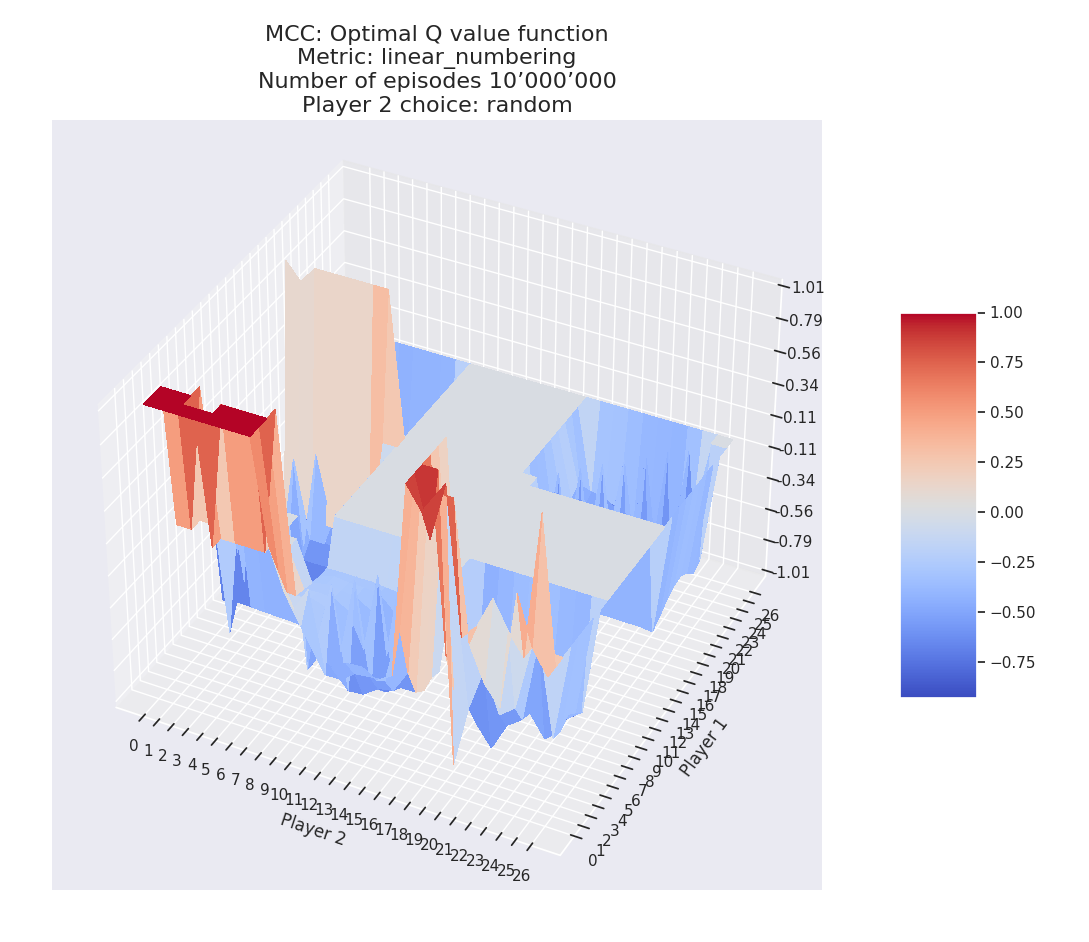
\includegraphics[width=1\linewidth]{Figures/mcc_linear_numbering_10000000_random} 
        \caption[MCC linear numbering]{MCC linear numbering}
        \label{fig:mcc linear_numbering}
    \end{subfigure}
    \begin{subfigure}{0.5\textwidth}
        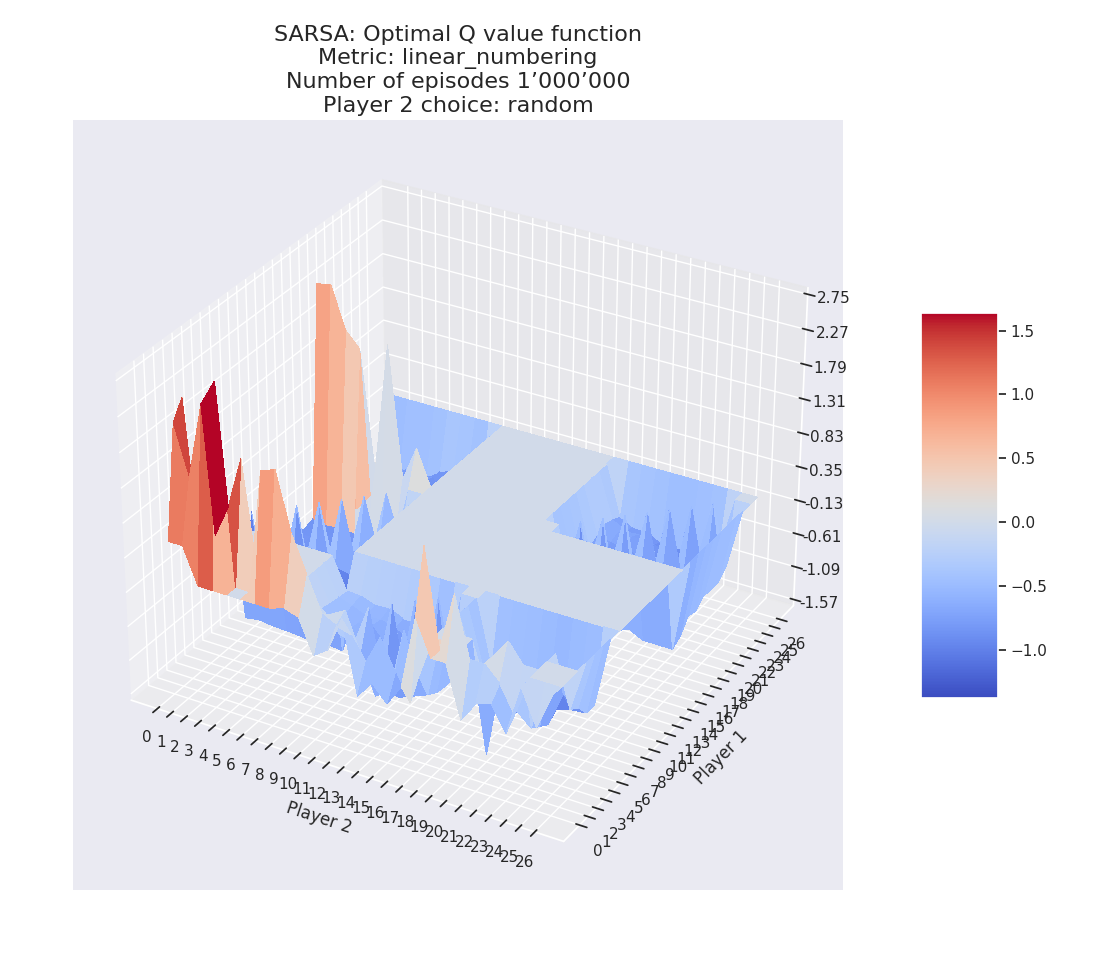
\includegraphics[width=1\linewidth]{Figures/SARSA_linear_numbering_1000000_random}
        \caption[SARSA linear numbering]{SARSA linear numbering}
        \label{fig:sarsa linear numbering}
    \end{subfigure} \\
    \caption{MCC and SARSA card encoding: linear numbering}
\label{fig:MCC and SARSA card encoding: linear numbering}
\end{figure}

\begin{figure}[ht!]
    \begin{subfigure}{0.5\textwidth}
        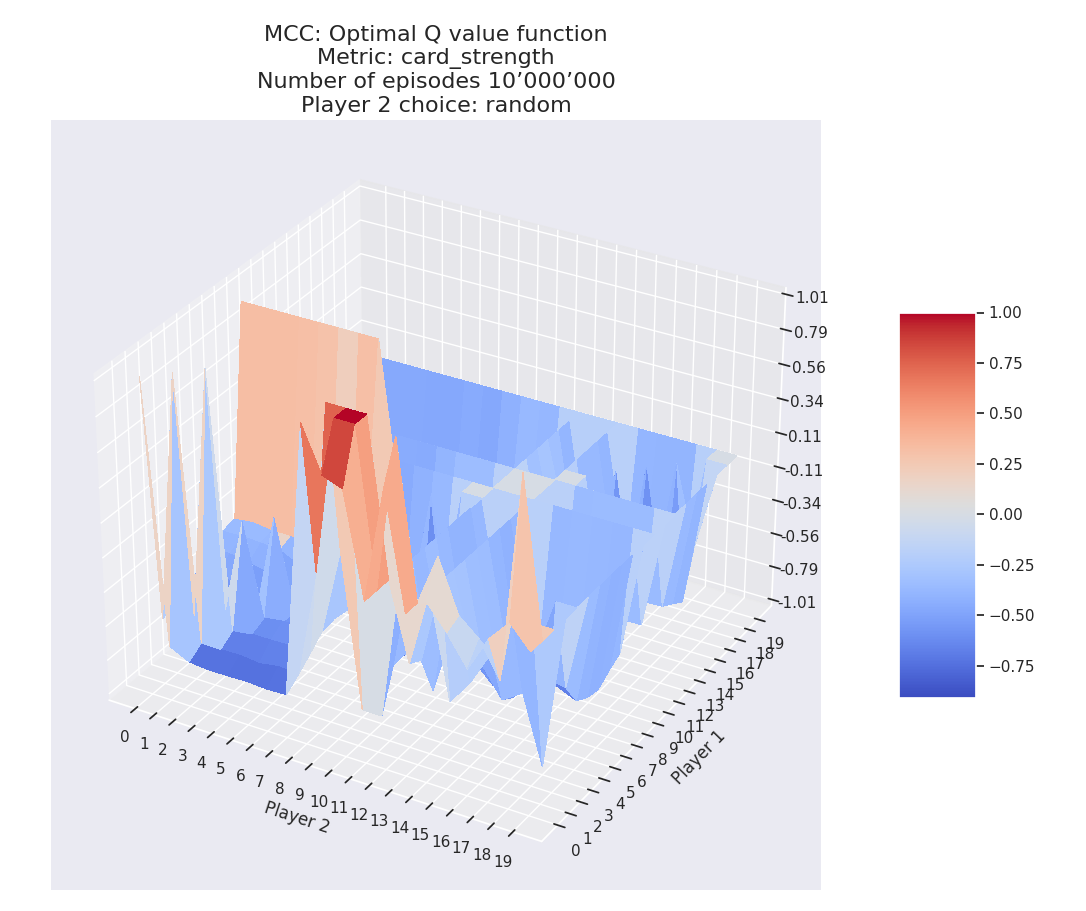
\includegraphics[width=1\linewidth]{Figures/mcc_card_strength_10000000_random} 
        \caption[MCC card strength]{MCC card strength}
        \label{fig:mcc card strength}
    \end{subfigure}
    \begin{subfigure}{0.5\textwidth}
        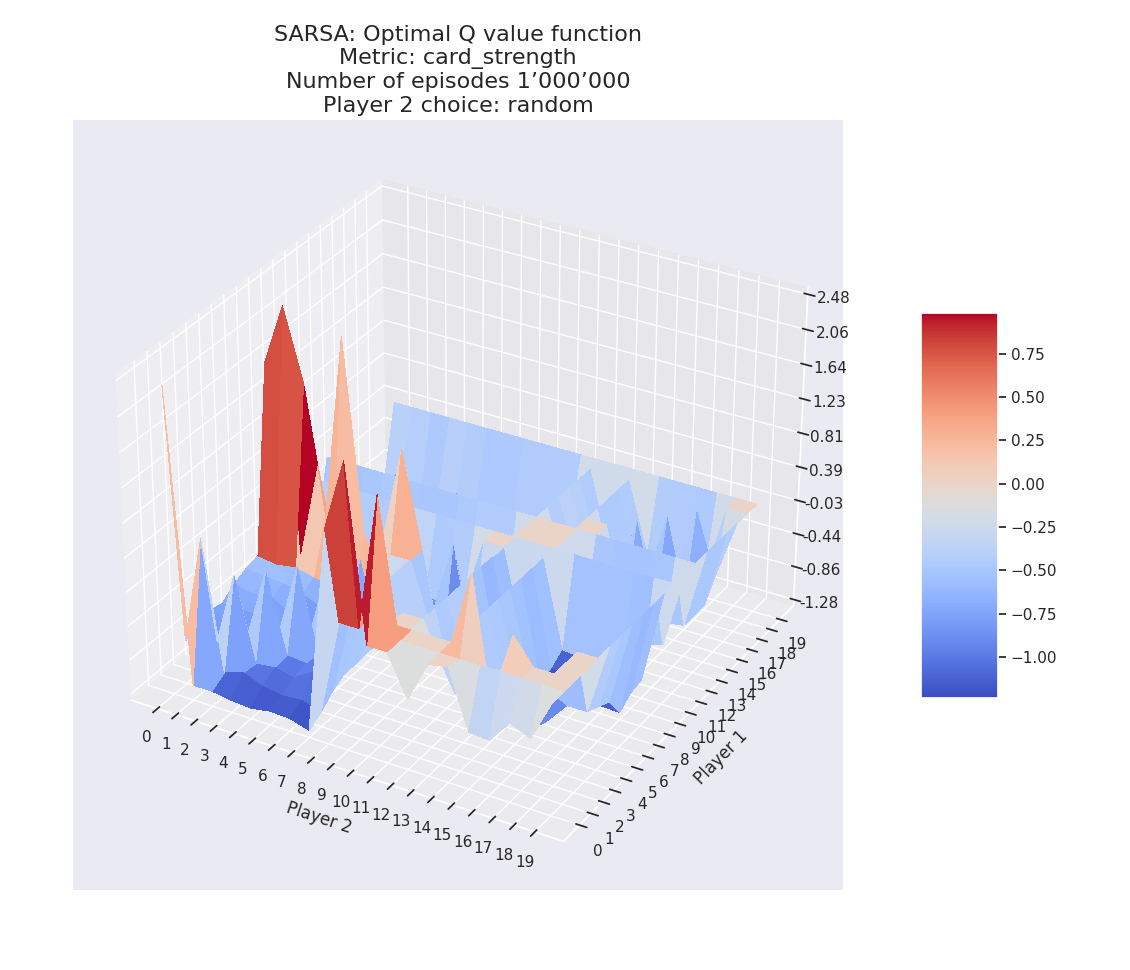
\includegraphics[width=1\linewidth]{Figures/SARSA_card_strength_1000000_random}
        \caption[SARSA card strength]{SARSA card strength}
        \label{fig:sarsa card strength}
    \end{subfigure} \\
    \caption{MCC and SARSA card encoding: card strength}
\label{fig:MCC and SARSA card encoding: card strength}
\end{figure}

\begin{figure}[ht!]
    \begin{subfigure}{0.5\textwidth}
        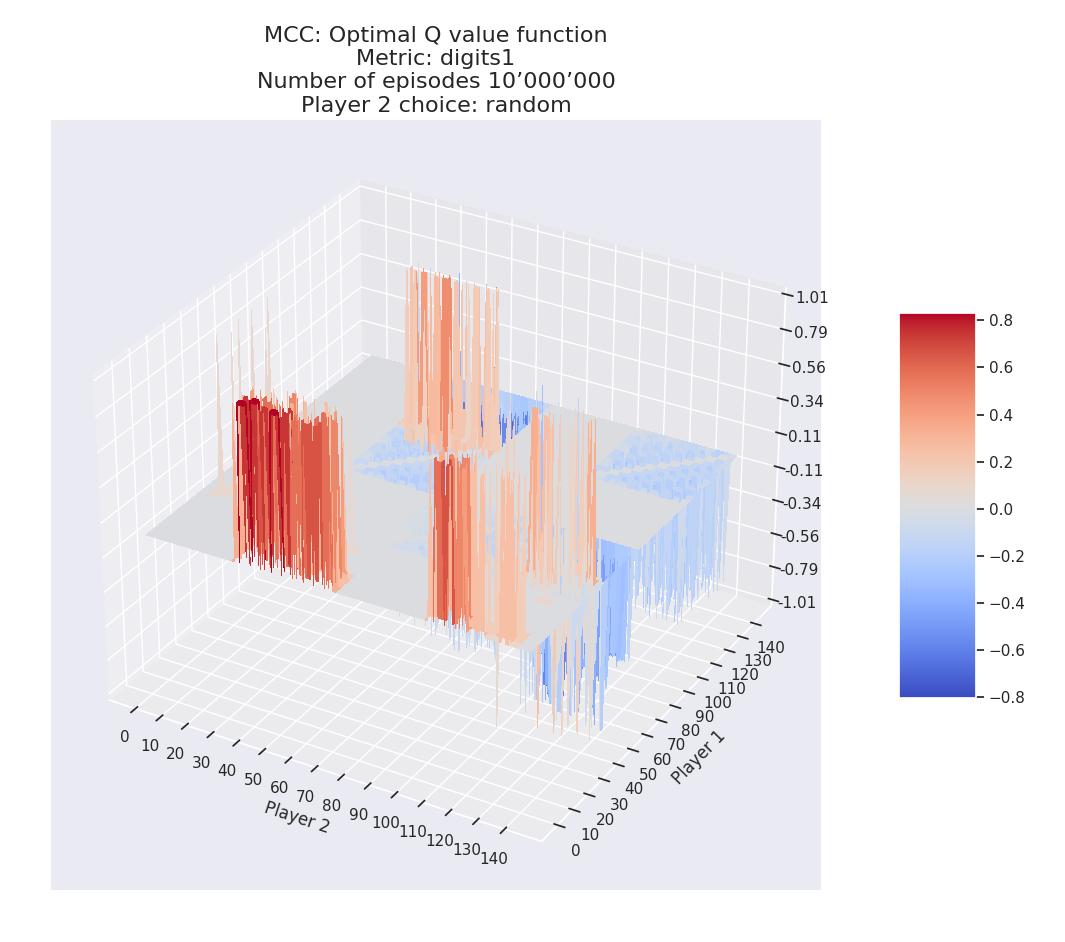
\includegraphics[width=1\linewidth]{Figures/mcc_digits1_10000000_random} 
        \caption[MCC digits1]{MCC digits1}
        \label{fig:mcc digits1}
    \end{subfigure}
    \begin{subfigure}{0.5\textwidth}
        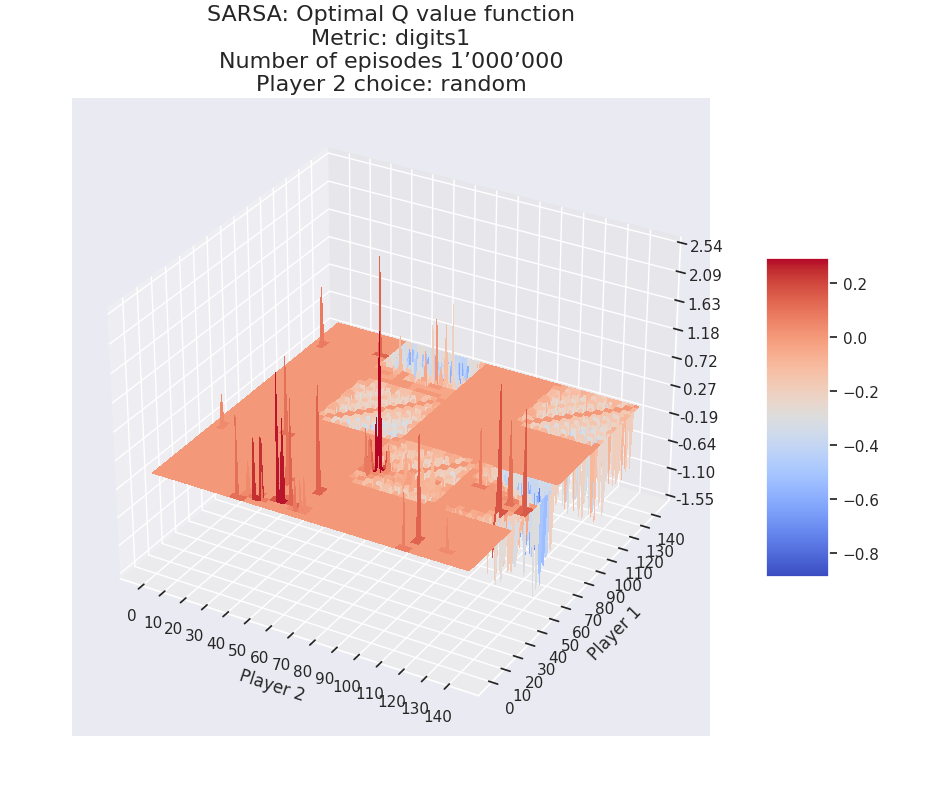
\includegraphics[width=1\linewidth]{Figures/SARSA_digits1_1000000_random}
        \caption[SARSA digits1]{SARSA digits1}
        \label{fig:sarsa digits1}
    \end{subfigure} \\
    \caption{MCC and SARSA card encoding: digits1}
\label{fig:MCC and SARSA card encoding: digits1}
\end{figure}

\begin{figure}[t!]
    \begin{subfigure}{0.5\textwidth}
        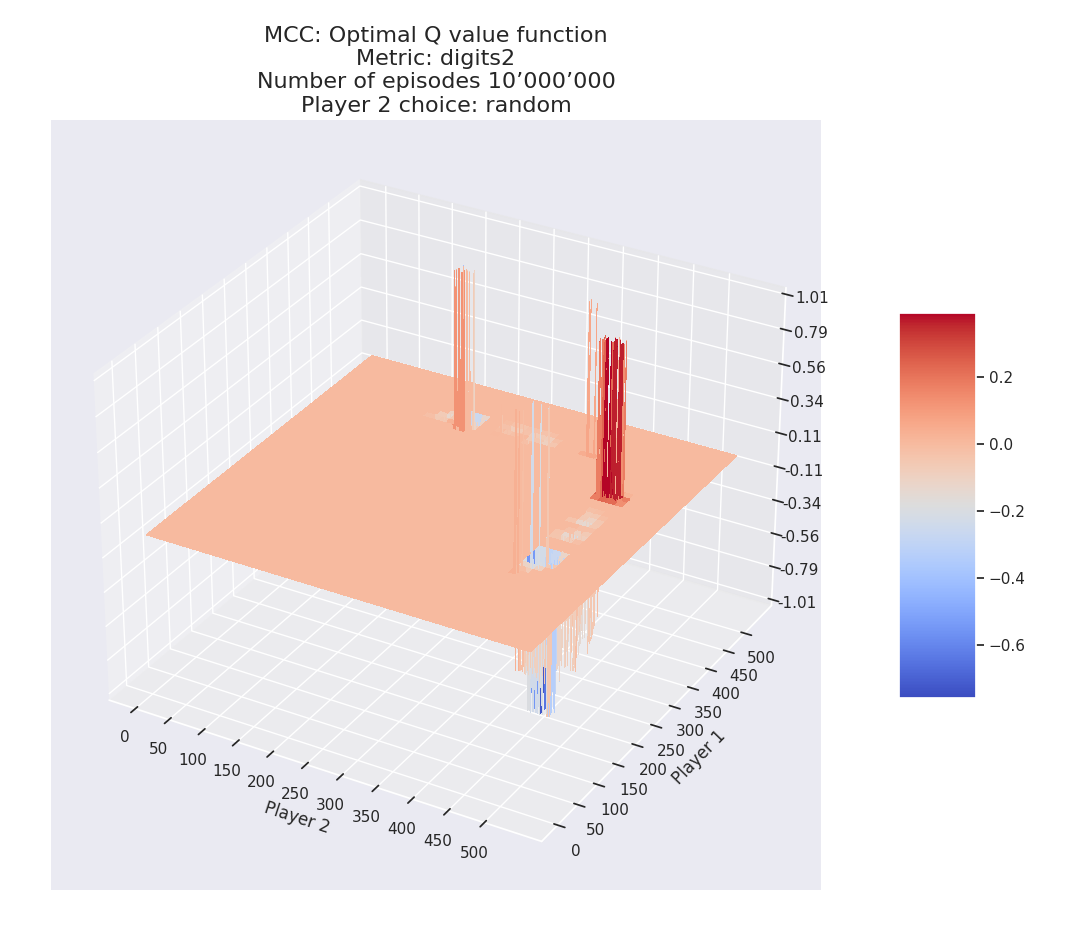
\includegraphics[width=1\linewidth]{Figures/mcc_digits2_10000000_random} 
        \caption[MCC digits2]{MCC digits2}
        \label{fig:mcc digits1}
    \end{subfigure}
    \begin{subfigure}{0.5\textwidth}
        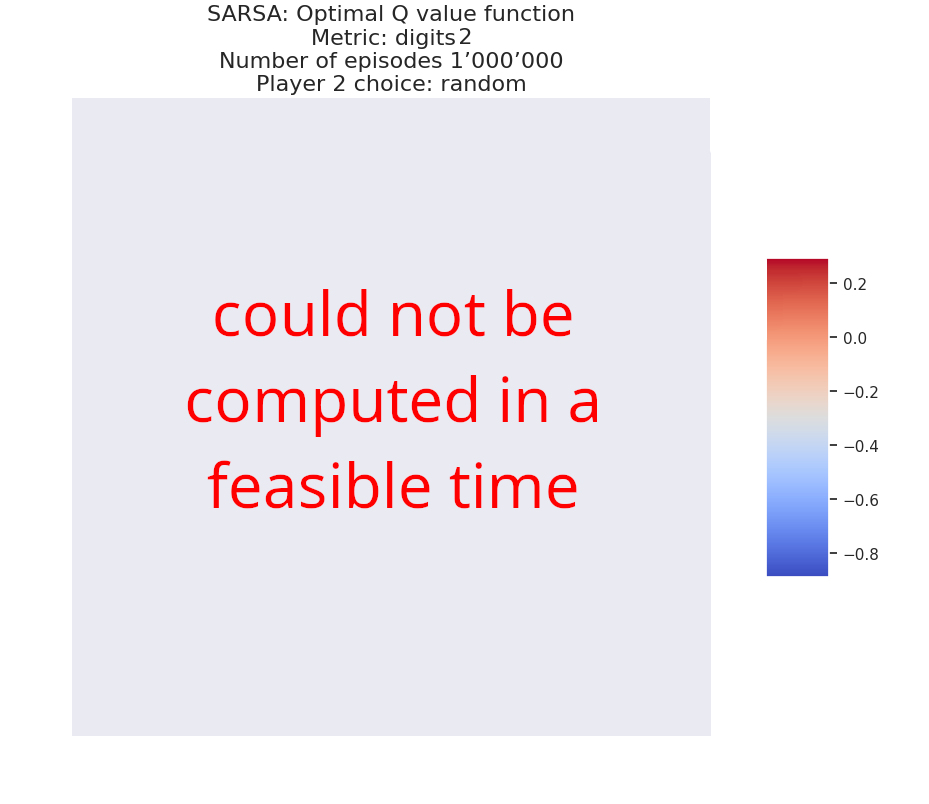
\includegraphics[width=1\linewidth]{Figures/SARSA_digits2_1000000_random}
        \caption[SARSA digits2]{SARSA digits2}
        \label{fig:sarsa digits2}
    \end{subfigure} \\
    \caption{MCC and SARSA card encoding: digits2}
\label{fig:MCC and SARSA card encoding: digits2}
\end{figure}
